\subsection{Opis}
			\par W pierwszym roku prowadzenia działalności mojej firmy będę jej jedynym pracownikiem. Będę odpowiedzialna za pozyskiwanie producentów, których produkty będą prezentowane na stronie, obsługą klientów, logistyką oraz będę się zajmować innymi działaniami niezbędnymi do prowadzenia sklepu internetowego. W trakcie rozwoju firmy planuję zatrudnienie pracowników, którzy przejmą ode mnie część obowiązków. Wprowadzając awanse pionowe, oznaczające pięcie się "w górę" na coraz to wyższe stanowiska w firmie, w drugim roku handlowiec awansuje na stanowisko starszego handlowca, robiąc tym samym lukę, co pozwala na zatrudnienie nowej osoby na stanowisko handlowca. Powielając ten schemat w trzecim roku, starszy handlowiec awansuje na stanowisko kierownika; handlowiec zostanie starszym handlowcem. W ten sposób można zatrudnić kolejną osobę, która zapełni lukę w hierarchii organizacyjnej przedsiębiorstwa. 
			 
			
			\begin{figure}[H]
				\centering
				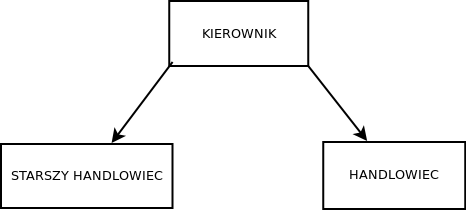
\includegraphics[scale=0.5]{struktura_org}
				\caption{Struktura organizacyjna przedsiębiorstwa}
				\label{search_pl}
			\end{figure}
			
			
		\subsubsection{Opis stanowisk pracy}
			\par Handlowiec
				\begin{itemize}
					\item telefoniczna i mailowa obsługa klienta
					\item obsługa zamówień 
					\item umieszczanie postów na portalach społecznościowych
					\item prowadzenie sprzedaży internetowej poprzez portale aukcyjne
					\item kompletowanie zamówień
			   	\end{itemize}
			
			\par Starszy handlowiec
				\begin{itemize}
					\item umieszczanie nowych produktów na stronie internetowej
					\item sporządzanie szczegółowych opisów produktów
					\item wystawianie faktur, paragonów
					\item kontakt z producentami
					\item kontrola procesu produkcji 
					\item organizowanie logistyki
				\end{itemize}	
					
			\par Kierownik
				\begin{itemize}
					\item pozyskiwanie nowych producentów mebli
					\item kreowanie oraz implementacja rozwiązań, które usprawnią sprzedaż internetową
					\item monitorowanie pracy handlowca i starszego handlowca
					\item monitorowanie rynku i konkurencji
					\item rozpatrywanie reklamacji
					\item delegowanie zadań podległym sobie pracownikom
				\end{itemize}

				
		\subsubsection{Wynagrodzenia}
			\par Przez "wynagrodzenie" rozumiemy ekwiwalent należny za pracę pracownika na rzecz pracodawcy w ramach stosunku pracy. W trakcie rozwoju firmy mam zamiar zatrudniać pracowników na postawie umowy o pracę. Wynagrodzenie początkowe jakie będzie otrzymywał pracownik, to wynagrodzenie minimalne, które zostało ujęte w kodeksie pracy. Na dzień dzisiejszy wynosi ono 2000 zł. brutto. Po otrzymanym awansie, pracownik będzie otrzymywał coraz wyższe wynagrodzenie adekwatne do zajmowanego stanowiska. Można przyjąć, iż będą to podwyżki na poziomie 20-30 \%.
			
			\par Jak powszechnie wiadomo wynagrodzenie pracownika pełni nie tylko funkcję czysto dochodową. Również bardzo ważną jest tu funkcja motywacyjna- im większy wpływ na swoją płacę ma pracownik, tym większą ma motywację do pracy. Dlatego bardzo ważne jest wprowadzenie systemu premii, nagród itp.. W moim przypadku może być to premia związana ze wzrostem sprzedaży, sumienności wykonywanych obowiązków, czy też zaangażowania w rozwój sklepu.
